\documentclass{article}

\usepackage{fancyhdr}
\usepackage{extramarks}
\usepackage{amsmath}
\usepackage{amsthm}
\usepackage{amsfonts}
\usepackage{tikz}
\usepackage{multicol}
\usepackage{float}
%\usepackage[plain]{algorithm}
\usepackage[ruled,vlined]{algorithm2e}
\usepackage{algpseudocode}

\usetikzlibrary{automata,positioning}

%
% Basic Document Settings
%

\topmargin=-0.45in
\evensidemargin=0in
\oddsidemargin=0in
\textwidth=6.5in
\textheight=9.0in
\headsep=0.25in

\linespread{1.1}

\pagestyle{fancy}
\lhead{\hmwkAuthorName}
\chead{\hmwkClass\ : \hmwkTitle}
\rhead{\firstxmark}
\lfoot{\lastxmark}
\cfoot{\thepage}

\renewcommand\headrulewidth{0.4pt}
\renewcommand\footrulewidth{0.4pt}

\setlength\parindent{0pt}

%
% Create Problem Sections
%

\newcommand{\enterProblemHeader}[1]{
    \nobreak\extramarks{}{Problem \arabic{#1} continued on next page\ldots}\nobreak{}
    \nobreak\extramarks{Problem \arabic{#1} (continued)}{Problem \arabic{#1} continued on next page\ldots}\nobreak{}
}

\newcommand{\exitProblemHeader}[1]{
    \nobreak\extramarks{Problem \arabic{#1} (continued)}{Problem \arabic{#1} continued on next page\ldots}\nobreak{}
    \stepcounter{#1}
    \nobreak\extramarks{Problem \arabic{#1}}{}\nobreak{}
}

\setcounter{secnumdepth}{0}
\newcounter{partCounter}
\newcounter{homeworkProblemCounter}
\setcounter{homeworkProblemCounter}{1}
\nobreak\extramarks{Problem \arabic{homeworkProblemCounter}}{}\nobreak{}

%
% Homework Problem Environment
%
% This environment takes an optional argument. When given, it will adjust the
% problem counter. This is useful for when the problems given for your
% assignment aren't sequential. See the last 3 problems of this template for an
% example.
%
\newenvironment{homeworkProblem}[1][-1]{
    \ifnum#1>0
        \setcounter{homeworkProblemCounter}{#1}
    \fi
    \section{Problem \arabic{homeworkProblemCounter}}
    \setcounter{partCounter}{1}
    \enterProblemHeader{homeworkProblemCounter}
}{
    \exitProblemHeader{homeworkProblemCounter}
}

%
% Homework Details
%   - Title
%   - Due date
%   - Class
%   - Section/Time
%   - Instructor
%   - Author
%

\newcommand{\hmwkTitle}{Homework\ \#4}
\newcommand{\hmwkDueDate}{Dec. 16, 2019}
\newcommand{\hmwkClass}{Modern Computational Statistics}
\newcommand{\hmwkClassTime}{ }
\newcommand{\hmwkClassInstructor}{}
\newcommand{\hmwkAuthorName}{\textbf{Huang Daoji}}

%
% Title Page
%

\title{
    \vspace{2in}
    \textmd{\textbf{\hmwkClass:\ \hmwkTitle}}\\
    \normalsize\vspace{0.1in}\small{Due\ on\ \hmwkDueDate\ at 3:10pm}\\
    \vspace{0.1in}\large{\textit{\hmwkClassInstructor\ \hmwkClassTime}}
    \vspace{3in}
}

\author{\hmwkAuthorName}
\date{}

\renewcommand{\part}[1]{\textbf{\large Part \Alph{partCounter}}\stepcounter{partCounter}\\}

%
% Various Helper Commands
%

% Useful for algorithms
\newcommand{\alg}[1]{\textsc{\bfseries \footnotesize #1}}

% For derivatives
\newcommand{\deriv}[1]{\frac{\mathrm{d}}{\mathrm{d}x} (#1)}

% For partial derivatives
\newcommand{\pderiv}[2]{\frac{\partial}{\partial #1} (#2)}

% Integral dx
\newcommand{\dx}{\mathrm{d}x}

% Alias for the Solution section header
\newcommand{\solution}{\textbf{\large Solution}}

% Probability commands: Expectation, Variance, Covariance, Bias
\newcommand{\E}{\mathrm{E}}
\newcommand{\Var}{\mathrm{Var}}
\newcommand{\Cov}{\mathrm{Cov}}
\newcommand{\Bias}{\mathrm{Bias}}

\begin{document}

%\maketitle

\pagebreak

\begin{homeworkProblem}

Similar to the proof in the LDA paper, we derive the ELBO for smoothed LDA first, then show the update formula for $\lambda, \gamma, \phi$

The ELBO for smoothed LDA is shown below, notice the first 5 terms are the same as LDA paper, and the last two are from the smoothed LDA assumption: $\beta \sim Dirichlet(\eta)$

\begin{equation}
    \begin{aligned}
        L(\lambda, \gamma, \phi; \alpha, \eta) &= \log p(w | \alpha, \eta) - KL(q(\beta, \theta, z | \lambda, \gamma, \phi) || p(\beta, \theta, z | w, \alpha, \eta)) \\
        &= E_{q} \log p(\theta | \alpha) + E_{q} \log p(z | \theta) + E_{q} \log p(w | z, \beta) - E_{q} \log q(\theta) - E_{q} \log q(z) \\
        &+ E_{q} \log p(\beta | \eta) - E_{q} \log q(\beta)
    \end{aligned}
\end{equation}

As shown in LDA paper appendix A.1(, and shown in class), Dirichlet distribution belongs to exponential family with natural parameter $\alpha - 1$ and sufifcient statistic $\log x$

\begin{equation}
    \begin{aligned}
        f(x | \alpha) &= \frac{1}{B(\alpha)} \prod x_{i}^{\alpha_{i} - 1} \\
        &= \exp\{\sum_{i} (\alpha_{i} - 1) \log x_{i} + \log \Gamma(\sum_{i} \alpha_{i}) - \sum_{i} \log \Gamma(\alpha_{i })\}
    \end{aligned}
\end{equation}

, and we have the below formula for exponential family.

\begin{equation}
    \frac{d}{{d \eta(\alpha)}} A(\alpha) = E_{p(x)} T(x)
\end{equation}

Thus, we show the explicit form for the sixth term

\begin{equation}
    \begin{aligned}
        E_{q} \log p(\beta | \eta) &= E_{q} \log \prod_{k} \frac{\Gamma(\sum_{i} \eta_{i})}{\prod_{i} \Gamma(\eta_i)} \prod_{i} \beta_{k, i}^{\eta_{i} - 1} \\
        &= K\log \Gamma(\sum_{i} \eta_i) - K \sum_{i} \log \Gamma(\eta_{i}) + \sum_{k} E_{q} [\sum_{i} (\eta_{i} - 1)\log \beta_{k, i}] \\
        &= K\log \Gamma(\sum_{i} \eta_i) - K \sum_{i} \log \Gamma(\eta_{i}) + \sum_{k} \sum_{i} (\eta_{i} - 1)E_{q} [\log \beta_{k, i}] \\
        &= K\log \Gamma(\sum_{i} \eta_i) - K \sum_{i} \log \Gamma(\eta_{i}) + \sum_{k} \sum_{i} (\eta_{i} - 1) \frac{d}{d \lambda_{k, i}}(\log \Gamma(\lambda_{k, i}) - \log \Gamma(\sum_{j} \lambda_{k, j})) \\
        &= K\log \Gamma(\sum_{i} \eta_i) - K \sum_{i} \log \Gamma(\eta_{i}) + \sum_{k} \sum_{i} (\eta_{i} - 1)(\Psi(\lambda_{k, i}) - \Psi(\sum_{j} \lambda_{k, j}))
    \end{aligned}
\end{equation}

Similarly, we have

\begin{equation}
    \begin{aligned}
        E_{q} \log p(\theta | \alpha) &= \log \Gamma(\sum_{i} \alpha_{i}) - \sum_{i} \log \Gamma(\alpha_{i}) + \sum_{i}(\alpha_{i} - 1)(\Psi(\gamma_{i}) - \Psi(\sum_{j} \gamma_{j})) \\
        E_{q} \log p(z | \theta) &= \sum_{d} \sum_{n}\sum_{i}\phi_{d, n, i}(\Psi(\gamma_{d, i}) - \Psi(\sum_{j} \gamma_{d, j})) \\
        E_{q} \log p(w | z, \beta) &= \sum_{d} \sum_{n} \sum_{i} \sum_{j} \phi_{d, n, i} w_{d, n, j} (\Psi(\lambda_{k, j}) - \Psi(\sum_{k} \lambda_{i, k})) \\
        E_{q} \log q(\theta) &= \sum_{d}(\log \Gamma(\sum_{j} \gamma_{d, j}) - \sum_{i} \log \Gamma(\gamma_{d, i}) + \sum_{i}(\gamma_{d, i} - 1)(\Psi(\gamma_{d, i}) - \Psi(\sum_{j} \gamma_{d, j}))) \\
        E_{q} \log q(z) &= \sum_{d} \sum_{n} \sum_{i} \phi_{d, n, i} \log \phi_{d, n, i} \\
        E_{q} \log q(\beta) &= \sum_{k}( \log \Gamma(\sum_{i} \lambda_{k, i}) - \sum_{i} \log \Gamma(\lambda_{k, i}) +  \sum_{i}(\lambda_{k, i} - 1)(\Psi(\lambda_{k, i}) - \Psi(\sum_{j} \lambda_{k, j})))
    \end{aligned}
\end{equation}

\textbf{(1)}

We take the relevant terms w.r.t. $\phi_{d, n, i}$ with a Lagrange multiplier $\lambda(\sum_{i} \phi_{d, n, i} - 1)$, since $\sum_{i} \phi_{d, n, i} = 1$

\begin{equation}
    \begin{aligned}
        L &= \phi_{d, n, i}(\Psi(\gamma_{d, i}) - \Psi(\sum_{j} \gamma_{d, j})) \\
        &+ \phi_{d, n, i} \sum_{j} w_{d, n, j} (\Psi(\lambda_{k, j}) - \Psi(\sum_{k} \lambda_{i, k})) \\
        &- \phi_{d, n, i} \log \phi_{d, n, i} \\
        &+ \lambda(\sum_{i} \phi_{d, n, i} - 1) \\
    \end{aligned}
\end{equation}

and set it to zero, we have

\begin{equation}
    \phi_{d, n, i} \propto \exp(\Psi(\gamma_{d, i}) - \Psi(\sum_{j} \gamma_{d, j}) + \sum_{j} w_{d, n, j} (\Psi(\lambda_{k, j}) - \Psi(\sum_{k} \lambda_{i, k}))),
\end{equation}

the $\Psi(\sum_{j} \gamma_{d, j})$ term could be removed, since it is constant for fixed $d$, thus does not matter after normalizing $\phi$. Similarly, we have

\begin{equation}
    \begin{aligned}
        \lambda_{i} &= \eta + \sum_{d} \sum_{n} \phi_{d, n, i} w_{d, n} \\
        \gamma_{d} &= \alpha + \sum_{n} \phi_{d, n, i}
    \end{aligned}
\end{equation}

\textbf{(2)}

Already shown in Equation(1, 4, 5)

\textbf{(3), (4)}

We show below the negative ELBO as a function of epoch and batch size
\begin{itemize}
    \item Batched LDA's performance is greatly influenced by initialization, while full-batched LDA is not
    \item full batched LDA outperforms batched version consistently, almost regradless of initialization
\end{itemize}

\begin{figure}[H]
    \centering
  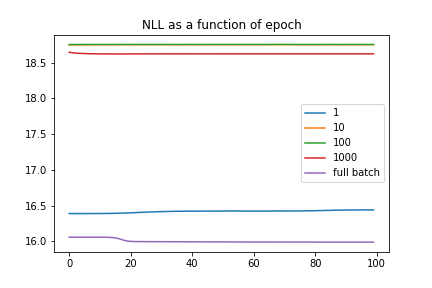
\includegraphics[width=0.4\linewidth]{./NLL_LDA.png}
  \caption{results of ELBO}\label{fig:awesome_image3}
\end{figure}


\end{homeworkProblem}


\begin{homeworkProblem}

\textbf{(1)}

The ELBO for logistic regression is

\begin{equation}
    \begin{aligned}
        L(\mu, \sigma^2) &= E_{q} \log p(x, \beta) - \log q(\beta | \mu, \sigma^2) \\
        \nabla_{\mu, \sigma^2} L &= \nabla_{\mu, \sigma^2} \int q(\beta, | \mu, \sigma^2) (\log p(x, \beta) - \log q(\beta | \mu, \sigma^2)) d\beta \\
        &= \int q(\beta | \mu, \sigma^2) \nabla_{\mu, \sigma^2} \log q(\beta, | \mu, \sigma^2) (\log p(x, \beta) - \log q(\beta | \mu, \sigma^2)) \\
        &- q(\beta | \mu, \sigma^2) \nabla_{\mu, \sigma^2} \log q(\beta, | \mu, \sigma^2) d\beta \\
        &= E_{q} \nabla_{\mu, \sigma^2} \log q(\beta | \mu, \sigma^2) (\log p(x, \beta) - \log q(\beta | \mu, \sigma^2) - 1) \\
        &= E_{q} \nabla_{\mu, \sigma^2} \log q(\beta | \mu, \sigma^2) (\log p(x, \beta) - \log q(\beta | \mu, \sigma^2)) \\
        \log p(x, \beta) &= \sum_{i} y_{i} \log \sigma(\beta^{T} x_{i}) + (1 - y_{i}) \log (1 - \sigma(\beta^{T} x_{i})) + \log N(\beta | 0, 1) \\
        \log q(\beta | \mu, \sigma^2) &= \log N(\beta | \mu, \sigma^2) \\
    \end{aligned}
\end{equation}

Now we only need to solve for $\nabla_{\mu, \sigma^2} \log q(\beta | \mu, \sigma^2)$.

\begin{equation}
    \begin{aligned}
        \log q(\beta | \mu, \sigma^2) &= \log N(\beta | \mu, \sigma^2) \\
        &= -\frac{D\log \sigma^2}{2} - \frac{\|\beta - \mu\|_2}{2 \sigma^2} \\
        \nabla_{\mu_{i}} \log q(\beta | \mu, \sigma^2) &= \frac{\beta_{i} - \mu_{i}}{\sigma^2} \\
        \nabla_{\sigma^2} \log q(\beta | \mu, \sigma^2) &= -\frac{D}{2 \sigma^2} + \frac{\|\beta - \mu\|_2}{2(\sigma^2)^2} \\
    \end{aligned}
\end{equation}

By substituting the above equation into (9), we derive the score function estimator for the gradient of ELBO w.r.t. $\mu$ and $\sigma$.

\textbf{(2)}

We use $\nabla_{\mu, \sigma^2} \log q(\beta, | \mu, \sigma^2)$ to control variation, which is also adopted in BBVI paper.

As for implementation details, I used Adam for optimizing BBVI(vanilla bbvi), BBVI with control variates(bbvi cv) and BBVI with reparameterization trick(bbvi rt). The results in ELBO(log -ELBO) are shown below.

\begin{figure}[!htb]
    \centering
  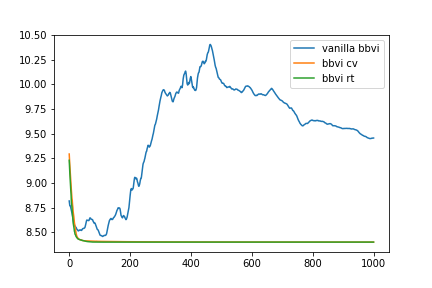
\includegraphics[width=0.5\linewidth]{./bbvi_full_batch_nll.png}
  \caption{results of various BBVI}\label{fig:awesome_image3}
\end{figure}

\textbf{(3)}

We have

\begin{equation}
    \begin{aligned}
        \nabla_{\mu, \sigma^2}L &= \nabla_{\mu, \sigma^2} E_{q} \log p(x, \beta) - \log q_{\mu, \sigma^2}(\beta) \\
        &= E_{q(\epsilon)} \nabla_{\mu, \sigma^2} \log p(x, g_{\mu, \sigma^2}(\epsilon)) - \log q_{\mu, \sigma^2}(g_{\mu, \sigma^2}(\epsilon)) \\
    \end{aligned}
\end{equation}

For logistic regression, we have (note that $\sigma$ is short for $\sigma((\mu + \sigma \epsilon)^{T} x_{i})$ except in $\mu + \sigma \epsilon$)

\begin{equation}
    \begin{aligned}
        \log p(x, g_{\mu, \sigma^2}(\epsilon)) &= \sum_{i} y_i \log \sigma + (1 - y_i) \log (1 - \sigma) + \log N(\mu + \sigma \epsilon | 0, 1) \\
        \nabla_{\mu} \log p(x, g_{\mu, \sigma^2}(\epsilon)) &= \sum_{i} y_i \frac{\sigma (1 - \sigma)}{\sigma} x_{i} + (1 - y_{i}) \frac{-\sigma (1 - \sigma)}{1 - \sigma} x_{i} - (\mu + \sigma \epsilon) \\
        &= \sum_{i} y_{i} (1 - \sigma) x_{i} + (y_{i} - 1) \sigma x_{i} - (\mu + \sigma \epsilon) \\
        \nabla_{\sigma^2} \log p(x, g_{\mu, \sigma^2}(\epsilon)) &= \{\sum_{i} y_{i} \frac{\sigma (1 - \sigma)}{\sigma} \epsilon x_{i} + (1 - y_{i}) \frac{- \sigma (1 - \sigma)}{1 - \sigma} \epsilon x_{i} - (\mu + \sigma \epsilon) \epsilon \} \frac{d \sigma}{d (\sigma^2)} \\
        &=  (\sum_{i} y_{i} (1 - \sigma) x_{i} + (y_{i} - 1) \sigma x_{i} - (\mu + \sigma \epsilon)) \frac{\epsilon}{2\sqrt{\sigma^2}} \\
        \log q_{\mu, \sigma^2}(g_{\mu, \sigma^2}(\epsilon)) &= \log N(\mu + \sigma \epsilon | \mu, \sigma^2) \\
        &= -\frac{D}{2}\log \sigma^{2} + C \\
        \nabla_{\sigma^2} \log q_{\mu, \sigma^2}(g_{\mu, \sigma^2}(\epsilon)) &= -\frac{D}{2 \sigma^2} \\
    \end{aligned}
\end{equation}

The results of BBVI with reparameterization trick is shown in \textbf{(2)}. Here we show the performance in minibatch senario.

\begin{figure}[H]
\minipage{0.33\textwidth}
  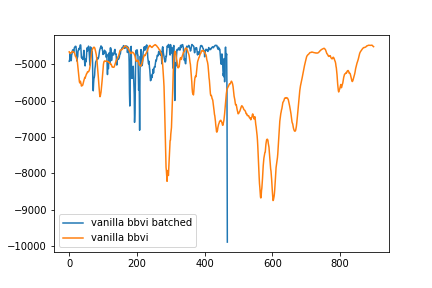
\includegraphics[width=\linewidth]{./bbvi_comp_vanilla.png}
  \caption{results of vanilla BBVI}\label{fig:awesome_image1}
\endminipage\hfill
\minipage{0.33\textwidth}%
  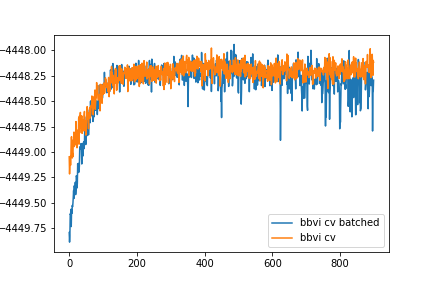
\includegraphics[width=\linewidth]{./bbvi_comp_cv.png}
  \caption{results of BBVI cv}\label{fig:awesome_image3}
\endminipage\hfill
\minipage{0.33\textwidth}%
  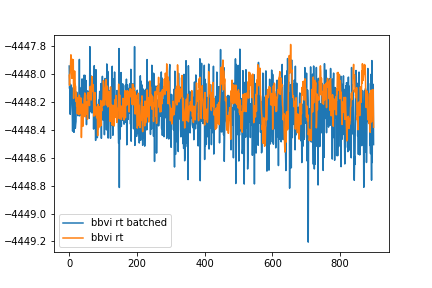
\includegraphics[width=\linewidth]{./bbvi_comp_rt.png}
  \caption{results of BBVI rt}\label{fig:awesome_image3}
\endminipage
\end{figure}

The settings are: batch size being 1000, sample result every 10 iteration $i.e.$ one epoch. Notice that vanilla BBVI diverged after 500 epoch even in such a large batch size. For BBVI with control variates and reparameterization trick, we only show their ELBO after 100 epoch to show their performance after convergence.

\textbf{(4)}

We show the result w.r.t. $Var(\mu)$ and $Var(\sigma)$ below. Notice that in my implementation, we estimate $\nabla_{\log \sigma^2}$ instead. As batch size increases, BBVI+CV/RT reduces the variances more and the variance becomes more stable.


\begin{figure}[H]
\minipage{0.24\textwidth}
  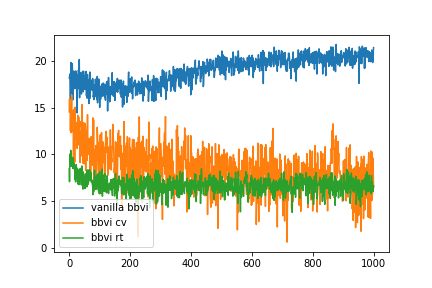
\includegraphics[width=\linewidth]{./bbvi_full_batch_var_mu_4.png}
  \caption{results of $\mu$, 4 samples}\label{fig:awesome_image1}
\endminipage\hfill
\minipage{0.24\textwidth}
  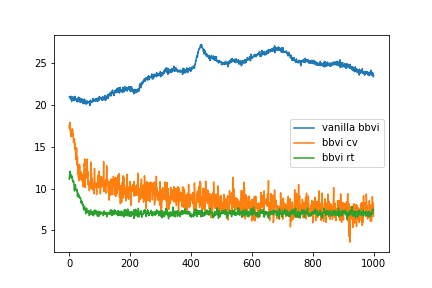
\includegraphics[width=\linewidth]{./bbvi_full_batch_var_mu_32.png}
  \caption{results of $\mu$, 32 samples}\label{fig:awesome_image1}
\endminipage\hfill
\minipage{0.24\textwidth}
  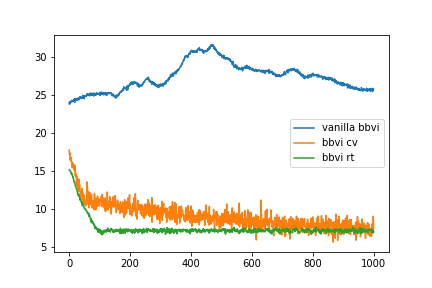
\includegraphics[width=\linewidth]{./bbvi_full_batch_var_mu_64.png}
  \caption{results of $\mu$, 64 samples}\label{fig:awesome_image1}
\endminipage\hfill
\minipage{0.24\textwidth}
  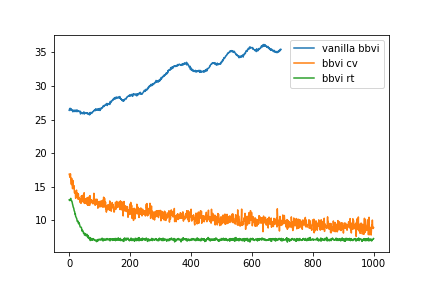
\includegraphics[width=\linewidth]{./bbvi_full_batch_var_mu_128.png}
  \caption{results of $\mu$, 128 samples}\label{fig:awesome_image1}
\endminipage
\end{figure}

\begin{figure}[H]
\minipage{0.24\textwidth}%
  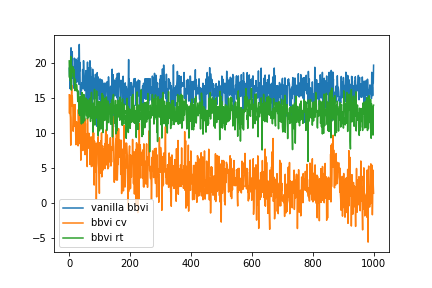
\includegraphics[width=\linewidth]{./bbvi_full_batch_var_sigma_4.png}
  \caption{results of $\sigma$, 4 samples}\label{fig:awesome_image3}
\endminipage \hfill
\minipage{0.24\textwidth}%
  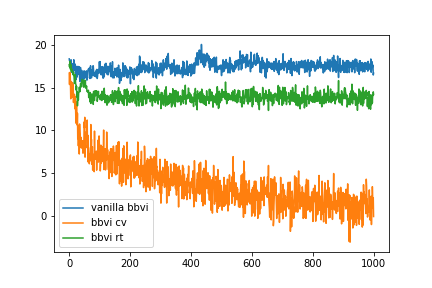
\includegraphics[width=\linewidth]{./bbvi_full_batch_var_sigma_32.png}
  \caption{results of $\sigma$, 32 samples}\label{fig:awesome_image3}
\endminipage \hfill
\minipage{0.24\textwidth}%
  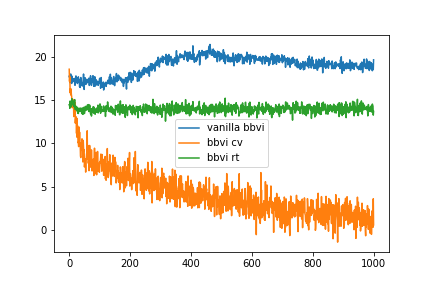
\includegraphics[width=\linewidth]{./bbvi_full_batch_var_sigma_64.png}
  \caption{results of $\sigma$, 64 samples}\label{fig:awesome_image3}
\endminipage \hfill
\minipage{0.24\textwidth}%
  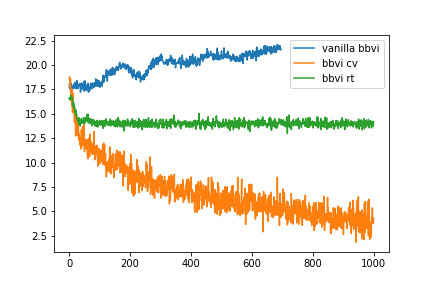
\includegraphics[width=\linewidth]{./bbvi_full_batch_var_sigma_128.png}
  \caption{results of $\sigma$, 128 samples}\label{fig:awesome_image3}
\endminipage
\end{figure}

\textbf{(6)}

NOTE: no better results made!
\begin{itemize}
    \item replace $\sigma$ with $\sigma_1, \sigma_2$ theortically should perform no worse than a single $\sigma$, but in practice not(ELBO drops to ~-1460)
    \item replace Gaussian prior by t-distribution or Laplace distribution does not work neither(ELBO drops to ~-1480)
\end{itemize}

\end{homeworkProblem}

\end{document}
